% POT.tex      pdflatex ZhCvGo15
% Diffuse globally, compute locally: a cyclist tale
% Tingnan Zhang, Daniel I. Goldman and Predrag Cvitanovi\'c

% \subsection{Periodic orbit theory}
% \label{s-POT}

\Po\ theory of deterministic diffusion, introduced in
\refrefs{art91,LorentzDiff}, exploits the fact that the periodic
Lorentz gas can be constructed by putting together translated copies
of an elementary cell.  Therefore quantities characterizing global
dynamics, such as the Lyapunov exponents and the diffusion tensor, can
be computed from the dynamics restricted to the elementary cell, as
shown numerically in \refref{CGS92}.

In \refrefs{art91,LorentzDiff,CGS92,Artuso94,CBdiffusion} it was shown
that deterministic diffusion tensor in the {\em periodic} Lorentz gas
can be expressed in terms of (relative) \po s, and exact formulae for
such global dynamical averages as Lyapunov exponent and diffusion
tensor were derived, using only the dynamics in the \emph{elementary
cell}, which we discuss now. For any dynamical system that has
translational symmetry, the full {\statesp} $\hM$ (\ie, both spatial
coordinates and momenta) has a periodic tiling
\[ %beq
\hM=\bigcup_{ \hn \in T} \pS_{\hn},
\] %eeq
by {\em translating} $\pS_{\hn}$ of an {\em elementary cell} $\pS$,
with $T$ the abelian group of lattice translations.

\begin{figure}[htbp]
	\begin{center}
    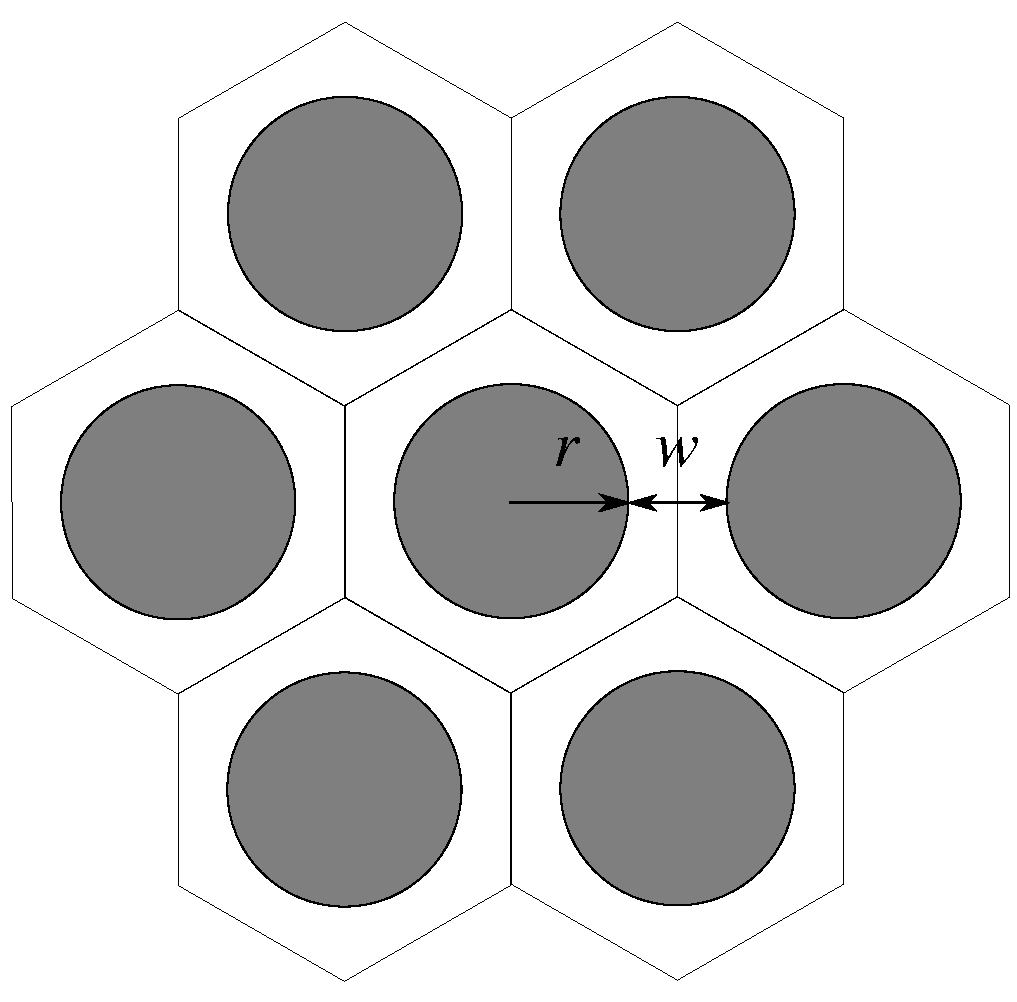
\includegraphics[width=0.25\textwidth]{diffuseLorentzGasParams}
	\end{center}
	\caption[]{\label{fig-LorentzGasParams}
        An elementary cell and its six unit translations. The ratio of
        distance $w$ between the nearest pair of disks to the    disk
        radius $r$ determines the dynamical properties in the system.
	}
	\TZ{2016-01-15}{This figure is also generated by me.}
\end{figure}

In the context of the triangular Lorentz gas system, an elementary
cell is the hexagon centered at a scatterer and lattice translations
$T$ applys only to spatial degrees of freedom, see
\reffig{fig-LorentzGasParams}. The dynamics restricted inside the
elementary cell is treated as the periodic boundary condition: when
the particle leaves the edge of the hexagon cell, it immediately
enters the region again from the opposite edge. The transition between
the finite and the infinite horizon is controlled by the ratio of $w/r$,
where $w$ is the gap between nearest pair of disk and $r$ the radius
of the disk. The horizon is finite for $w/r < 4/\sqrt{3}-2 =
0.3094\dots$.

    \PC{2013-02-03} { Roberto says we must incorporate kneading
    determinants from Cristadoro\rf{ArtCri03,Cristad06,CriKnDeEsp12}.
    }

%    \PC{2015-10-21}
%    {edits based Cvitanovi\'c,  Eckmann,and Gaspard\rf{LorentzDiff}}
%In \refrefs{art91,LorentzDiff,CGS92,Artuso94,CBdiffusion}  an explicit
%connection between the global diffusion and the dynamics restricted to
%an elementary cell.
%Our method applies to any  hyperbolic dynamical system that is
%a periodic tiling $\hM=\bigcup_{ \hn \in T} M_{
%\hn}$
%of the dynamical phase space $\hM$ by {\sl translates}
%$M_{\hn}$
%of an {\sl elementary cell} $M$, with $T$ the abelian group of lattice
%translations.
%Furthermore, each elementary cell may be built from a
%{\sl fundamental domain}
%$\tM$
%by the action of a discrete (not necessarily Abelian) group $G$.

\PC{2014-11-18}{reinstate mass, velocity, size to get $\beta$, $m$,
$\sigma$ dependencies right?}

Previous works by Machta and Zwanzig\rf{MacZwa83} have given numerical
results for the diffusion constant in Lorentz gases,  as well as
estimates based on a random walk approximation. We shall follow their
notation and fix the radius of the disks to 1, and assume unit
particle speed.

Let $\hx(t)\,=\,\hflow{t}{\hx_0}$ denotes the point in the full
space $\hM$ reached by the flow in time $t$.
$x(t)\,=\,\flow{t}{\xInit}$ denotes the corresponding flow in the
elementary cell; the two are related by
\beq
\hn_t(\xInit)=\hflow{t}{\xInit} - \flow{t}{\xInit} \in T \,,
\ee{l-diff-hatn1}
the translation of the endpoint of the global path into the elementary
cell $\pS$. The diffusion tensor, by definition, is the temporal and
ensemble average of the displacement:
\beq
D_{ij} =
\lim_{t\to\infty}\frac{1}{2dt}\left\langle\hn_t(\xInit)_i\hn_t(\xInit)_j\right\rangle_{\hM}\,,
\label{eq-diff-def}
\eeq
where the index $i$ and $j$ are restricted to the spatial components
$q_i$ of the {\statesp} vectors $x=(q,p)$, \ie, if the dynamics is
Hamiltonian, the sum is over the $d$ degrees of freedom.

Following the general definition \refeq{eq-diff-def}, one can
numerically compute the diffusion coeffcient for various systems
(which is not limited to the Lorentz gas). However, little insight is
gained in the dynamics of the system. Instead,
\cite{art91,LorentzDiff,CGS92,Artuso94,CBdiffusion} suggest we study
the quantity
\beq
Q(\beta)\,=\, \lim_{t \rightarrow \infty} \frac{1}{t} \log
\langle e^{\beta \cdot \hn_t(x)} \rangle_{\hM} ~, \quad
\label{eq-diff-1}
\eeq
where $\beta$ is an auxiliary vector quantity. The interesting
dynamical averages such like mean drift and diffusion can be easily
obtained by taking derivatives of $Q(\beta)$ and set $\beta =
0$, e.g.:
\bea
2d D_{ij} &=& \left . {\frac{\partial}{\partial \beta_i}} {\frac{\partial}
{\partial \beta_j}} Q(\beta)\right\vert_{\beta=0}\\\nonumber
&=&\lim_{t\rightarrow
\infty} {\frac{1}{t}} \langle {\hn_t(x)_i \hn_t(x)_j } \rangle_{\hM} \,,
\eea
yields a diffusion matrix.  The diffusion tensor matrix can, in
general, be anisotropic (\ie, have $d$ distinct eigenvalues and
eigen\-vectors). The spatial diffusion constant is then given by the
Einstein relation
\beq
D\,=\,{1\over 2 d} \sum_i^d \left .{{\partial}^2 \over {\partial
\beta^2_i}} Q(\beta)\right |_{\beta=0} \,=\, \lim_{t\rightarrow
\infty} {1\over{2d t}} \langle {(\hat{q}(t) -q)^2 } \rangle_{\hM}~ ~,
\eeq

Because of the translational invariance, it was shown in \refref{CGS92}
that the ensemble average in~\refeq{eq-diff-1} can be written as an
integral over the elementary cell
\beq
\langle e^{\beta\cdot(\hx(t)-x)} \rangle
   = \frac{1}{\vert \pS \vert}\int_{x,y\in \pS} dxdy {\cal L}^t(y,x),
\eeq
given the \evOper
\beq
{\cal L}^t(y,x) = e^{\beta\cdot(\hx(t)-x)}\delta(y-x(t))\,,
\label{eq-evo-flow}
\eeq
for the flow. It is a linear operator such that it satisfies the
semi-group property:
\beq
{\cal L}^{t_1+t_2}(y,x) = \int dx^{\prime} {\cal
L}^{t_2}(y,x^{\prime}) {\cal L}^{t_1}(x^{\prime},x)
\eeq
and when $\beta = 0$ it reduces to the Ruelle-Perron-Frobenius
operator.

We may also introduce the same operator for discrete maps, after we
have chosen the appropriate Poincar\'e section and study the dynamics
restricted to the intersections of the flow on the hyper-surface:
\beq
{\cal L}^n(y,x) = e^{\beta\cdot(\hat{f}^n(x)-x)}\delta(y-f^n(x))\,.
\label{eq-evo-map}
\eeq

For the Lorentz gas system, consider the Poincar\'e section to be the
edge of the disk.  The finite horizon guarantees that the particle
will collide with a disk in finite time and the Poincar\'e map is
truly a ``return map''. Once we have specified the arch length
$\varphi$ at which the particle hits the disk and the incident angle
$\psi$ (which gives the tangent velocity component at the collision
point), the dynamics is fully determined. There are two other marginal
directions along which the dynamics is trivial, because the system is
Hamiltonian.

The dynamical average we are interested does not belong to any
particular finite time (or a finite number of returns on the section). As
$t\to\infty$ (or $n\to\infty$ for the map), the average quantities are
dominated by the leading eigenvalue of ${\cal L}^t$, $\lambda_0 =
e^{\eigenvL(\beta)}t$, \ie, it is straightforward to show that in the
limit $Q(\beta) \to \eigenvL(\beta)$.

For sake of simplicity, we will proceed with the derivation for the
return map and in the end generalize to the continuous flow. While the
evolution operator \refeq{eq-evo-flow} and \refeq{eq-evo-map} act on a
functional space of infinite dimension, their spectrum may still be
extracted by the trace formula:
\beq
\det(1-z{\cal L}) =
\exp\left(-\sum_{n=0}^{\infty}\frac{z^n}{n}\tr{\cal L}^n\right)\,,
\label{eq-det-disc-def}
\eeq
where $z$ is an auxiliary variable, and the trace:
\beq
\Tr{{\cal L}^n} = \int_{\pS}dx ~
e^{\beta\cdot(\hat{f}^n(x)-x)}\delta(x-f^n(x))\,.
\label{eq-trace-disc}
\eeq

With the $\delta$ functon inside, eq.~\refeq{eq-trace-disc} picks up a
contribution whenever $x = f^n(x)$, e.g. when $x$ is a periodic point
of the map $f$. When $n$ is not a prime number, it is possible that
$x$ belongs to a periodic orbit $p$ of period $n_p$, and satisfies the
multiplicity $n_p r = n$, where $r$ is the number of repeats.

We may now restrict the integral only in the vicinities of the prime
periodic orbits (\ie, those who are not the repeat of other periodic
orbits) of the return map, and write:
\beq
\Tr{{\cal L}^n} = \sum_p\delta_{n,
n_pr}\sum_{x\in p}\frac{e^{r\beta\cdot\hat{n}_p(x)}}{\vert\det\left({\bf 1 -
J}_p^{r}(x)\right)\vert}\,,
\label{eq-trace-expan}
\eeq
where ${\bf J}_p(x) = Df^{n_p}(x)$ is the Jacobian. Using the chain
rule of differentiation, it follows that ${\bf J}_p(x) = {\bf J}_p $,
\ie, the Jacobian is independent of the point $x$ on the cycle. We
can also show that $\hn_p(x) = \hn_p$, by summing all the free
flights along the cycle: because translations are commutative, the
order at which individual displacements are added stays irrelevant.

With \refeq{eq-det-disc} and \refeq{eq-trace-disc}, we finally
obtain:
\beq
\det(1-z{\cal L}) = \prod_p \exp\left(-\sum_{r =
1}^{\infty}\frac{z^{n_p r}}{r}
\frac{e^{r\beta\cdot\hat{n}_p}}{\vert\det\left({\bf 1 -
J}_p^{r}\right)\vert}\right)\,,
\label{eq-det-disc}
\eeq
where the product runs over all prime periodic cycles in the
elementary cell.

Generalization to continuous time\rf{bowen,pexp} amounts to the
replacement
%$ z\,=\,e^{-s} $,
$ z^{n_p} \rightarrow e^{-s \period{p}} $, where $\period{p}$
is now the (not necessarily integer)
%{\sl time-}
period of the prime cycle $p$ for the flow. One has to distinguish the
period of the return map, $n_p$, which is the number of collisions for
the cycle, and the period of the flow, $\period{p}$, which represents
the time traveled after finishing the cycle once. The spectrum
determinant for the continuous time is:

\beq
Z(\beta, s)\,=\,\prod_{p\in\PP} \exp \left( - {
 \sum_{r=1}^\infty {1 \over r}
 { e^{(\beta \cdot \hn_p- s \period{p}) r } % z^{n_p r}
 \over { | \det \left( {\bf 1}-{\bf J}_p^{r} \right) | } }
 } \right)\,,
\label{eq-det-cont}
\eeq
and the associated dynamical zeta function:
\beq
1/\zeta(\beta, s)\,=\,\prod_{p}\left( 1 - \frac{e^{(\beta \cdot \hn_p-
      s \period{p})}}{|\ExpaEig_p|} \right) ~,
\label{eq-zeta-cont}
\eeq
if one approximates the $\left( {\bf 1}-{\bf J}_p^{r} \right) |$ with
the product product of expanding eigenvalues of the cycle,
$\ExpaEig_p$. The determinant~\refeq{eq-det-cont} has many resonances
(zeros) on the complex $s$ plane, even for the simplest systems.
According to previous literatures~\rf{DasBuch}, extracting the leading
eigenvalue of the evolution operator amounts to solve the implict
equation $Z(\beta, s(\beta)) = 0$. By taking derivatives with respect
to $\beta$ we arrive at
\beq
\frac{ds}{d\beta} = -\frac{\partial Z}{\partial\beta}/\frac{\partial
Z}{\partial s}\,.
\eeq
The final piece needed now is to determine the actual value $s(\beta)$
at $\beta = 0$. The Lorentz gas system is infinite and yet
\emph{bounded} such that the particle can never exist the lattice.
In other words, the flow is \emph{conserved}, and the escape rate
$s(\beta = 0) = 0$. The problem at hand is automatically resolved, and
also provides us a sanity check $Z(0, 0)\approx 0$, if the cycle
expansion formula is correct and all cycles are included.

The \dzeta\ \cycForm\ for the diffusion constant, zero mean drift
$ \expct{ \hat{x}_i } = 0 $ (because the system is symmetric), is
given by
 \beq
 D \,=\,{1 \over 2 d} { \expct{\hat{x}^2}_\zeta \over
 \expct{\period{}}_\zeta } \,=\,{1 \over 2 d } \, {1 \over
 \expct{\period{}}_\zeta} \sumprime \frac{(-1)^{k+1} (\hn_{p_1}+
 \cdots+ \hn_{p_k})^2} {|\ExpaEig_{p_1}\cdots \ExpaEig_{p_k}|} \, ,
\label{eq-diff-ec}
\eeq
where $\expct{\period{}}_\zeta = \partial Z/\partial s\vert_{s = 0}$,
and the sum is over all distinct non-repeating combinations of prime
cycles. The derivation is standard, still the formula is strange.
Diffusion is unbounded motion across an infinite lattice;
nevertheless, the reduction to the elementary cell enables us to
compute relevant quantities in the usual way, in terms of periodic
orbits.
